\section{Approximate inference}
\label{sec:approxinference}
Exact inference for \textbf{singly connected graphs} (i.e. those in which there's at most one undirected path between any nodes) has a time and space complexity which is linear in the size of the network. This is good for graphs like the famous \textit{Burglary Example}, but once we try inference on \textbf{multiply connected graphs}, we lose this nice property. Variable elimination can have \textbf{exponential time and space complexity} in the worst case, even when the number of parents per node is bounded. \cite{russel2010} So, what can we do? 
\subsection{Theoretical background}
\textbf{Approximate inference} is the answer. It consists in \textbf{randomized sampling algorithms} (also known as \textit{Monte Carlo}) that provide approximate answers having an accuracy depending on the number of samples generated. The obvious, first, step is \textbf{generating a sample} from a known probability distribution. This is basically how inference in real life is done: we run the experiment, count the results, compute the probabilities. It is also known as \textbf{stochastic approximation}, and for $\hat{N}\rightarrow N$ it will converge to the true probability. The standard deviation of the error in each probability will be proportional to $\frac{1}{\sqrt{n}}$.
\subsubsection{Rejection sampling}
\textbf{Rejection sampling} is probably the most straightforward way of proceeding. It can be used to compute conditional probabilities $P(X|e)$ by generating samples from the prior distribution, then \textbf{rejecting} those that do not match the evidence. Then, pretty easily, the estimate $\hat{P}(X=x|e)$ is obtained by counting how often $X=x$ occurs in the samples.
\subsubsection{Likelihood weighting}
Rejection sampling has a pretty notable downside: we are generating multiple samples that are inconsistent with our evidence, resulting in a non-trivial amount of wasted time. \textbf{Likelihood weighting} tries to solve that. The idea is simple: instead of throwing away the results that don't fit the evidence, we just weigh them less in the final count. The reason for doing that is simple: we would like to sample from the true posterior distribution, but usually this is too hard, as no polynomial-time approximation can exist. Now, a rather big question still has to be answered: \textit{how do we compute the weights?} The solution is just the product of the conditional probabilities for the evidence variables given their parents:
\begin{equation}
    w(\mathbf{z})=\alpha \prod_{i=1}^{m} P\left(e_{i} \mid \text { parents }\left(E_{i}\right)\right)
\end{equation}
This approach can be \textbf{much more efficient} than rejection sampling, though it will lose its performance when $n$ becomes higher: the noise that the low-weight samples add becomes more and more \textit{distracting} as the number of samples increases. We know, according to Hoeffding's inequality, that 
\begin{equation}
    P(|s-p|>\epsilon) \leq 2 e^{-2 n \epsilon^{2}}
\end{equation}
so we may be able to set an accuracy threshold for our approximate inference.
\subsection{Approximate inference in pgmpy}
As with any other interesting task, \texttt{pgmpy} allows us to perform these two. To keep things tidied up, a good idea would be creating a \texttt{SampleTester()} class having different methods for RS and LW. The processing method for rejection sampling would look like the following:
\begin{minted}{python}
def process_rs(self, size, evidence, query):
    rejection_sample = self.sampler.rejection_sample(evidence=evidence, size=size,
    return_type='recarray')[query]
    sample_probs = self.return_probs(rejection_sample)
    exact_result = self.exact_inference.query([query], dict(evidence)).values
    absolute_error = self.calculate_error(sample_probs, exact_result)
    return absolute_error
\end{minted}
while the one for likelihood weighting would be as follows:
\begin{minted}{python}
def process_lws(self, size, evidence, query):
    likelihood_sample = self.sampler.likelihood_weighted_sample(evidence=evidence,
    size=size, return_type='recarray')
    sample_probs = self.return_weighted_probs(likelihood_sample[query],
    likelihood_sample['_weight'])
    exact_result = self.exact_inference.query([query], dict(evidence)).values
    absolute_error = self.calculate_error(sample_probs, exact_result)
    return absolute_error
\end{minted}
Then, we just have to add some \textbf{utilities} for the error calculation and the sample counting:
\begin{minted}{python}
def return_probs(self, samples):
    # Get the unique values and their counts
    unique, counts = np.unique(samples, return_counts=True)
    # Divide the counts by the total number, getting a probability from 0 to 1
    counts = (counts/len(samples))
    # Zip the value and its probability in a dict
    return dict(zip(unique, counts)) 
def return_weighted_probs(self, samples, weights):
    unique = np.unique(samples)
    # Zero array for the weights sum, which we'll divide by the sum of weights
    counts = np.zeros(len(np.unique(samples))) 
    iterator = np.nditer(samples, flags=['f_index'])
    for value in iterator:
        counts[value] += weights[iterator.index]
    counts = (counts/np.sum(weights))
    # Zip the value and its probability in a dict
    return dict(zip(unique, counts)) 
\end{minted}
and that's it! We can test our methods with an example evidence $Safety=high,Maintenance=low$ and query the acceptability. The \textbf{results} are the following:
\begin{figure}[ht]
    \centering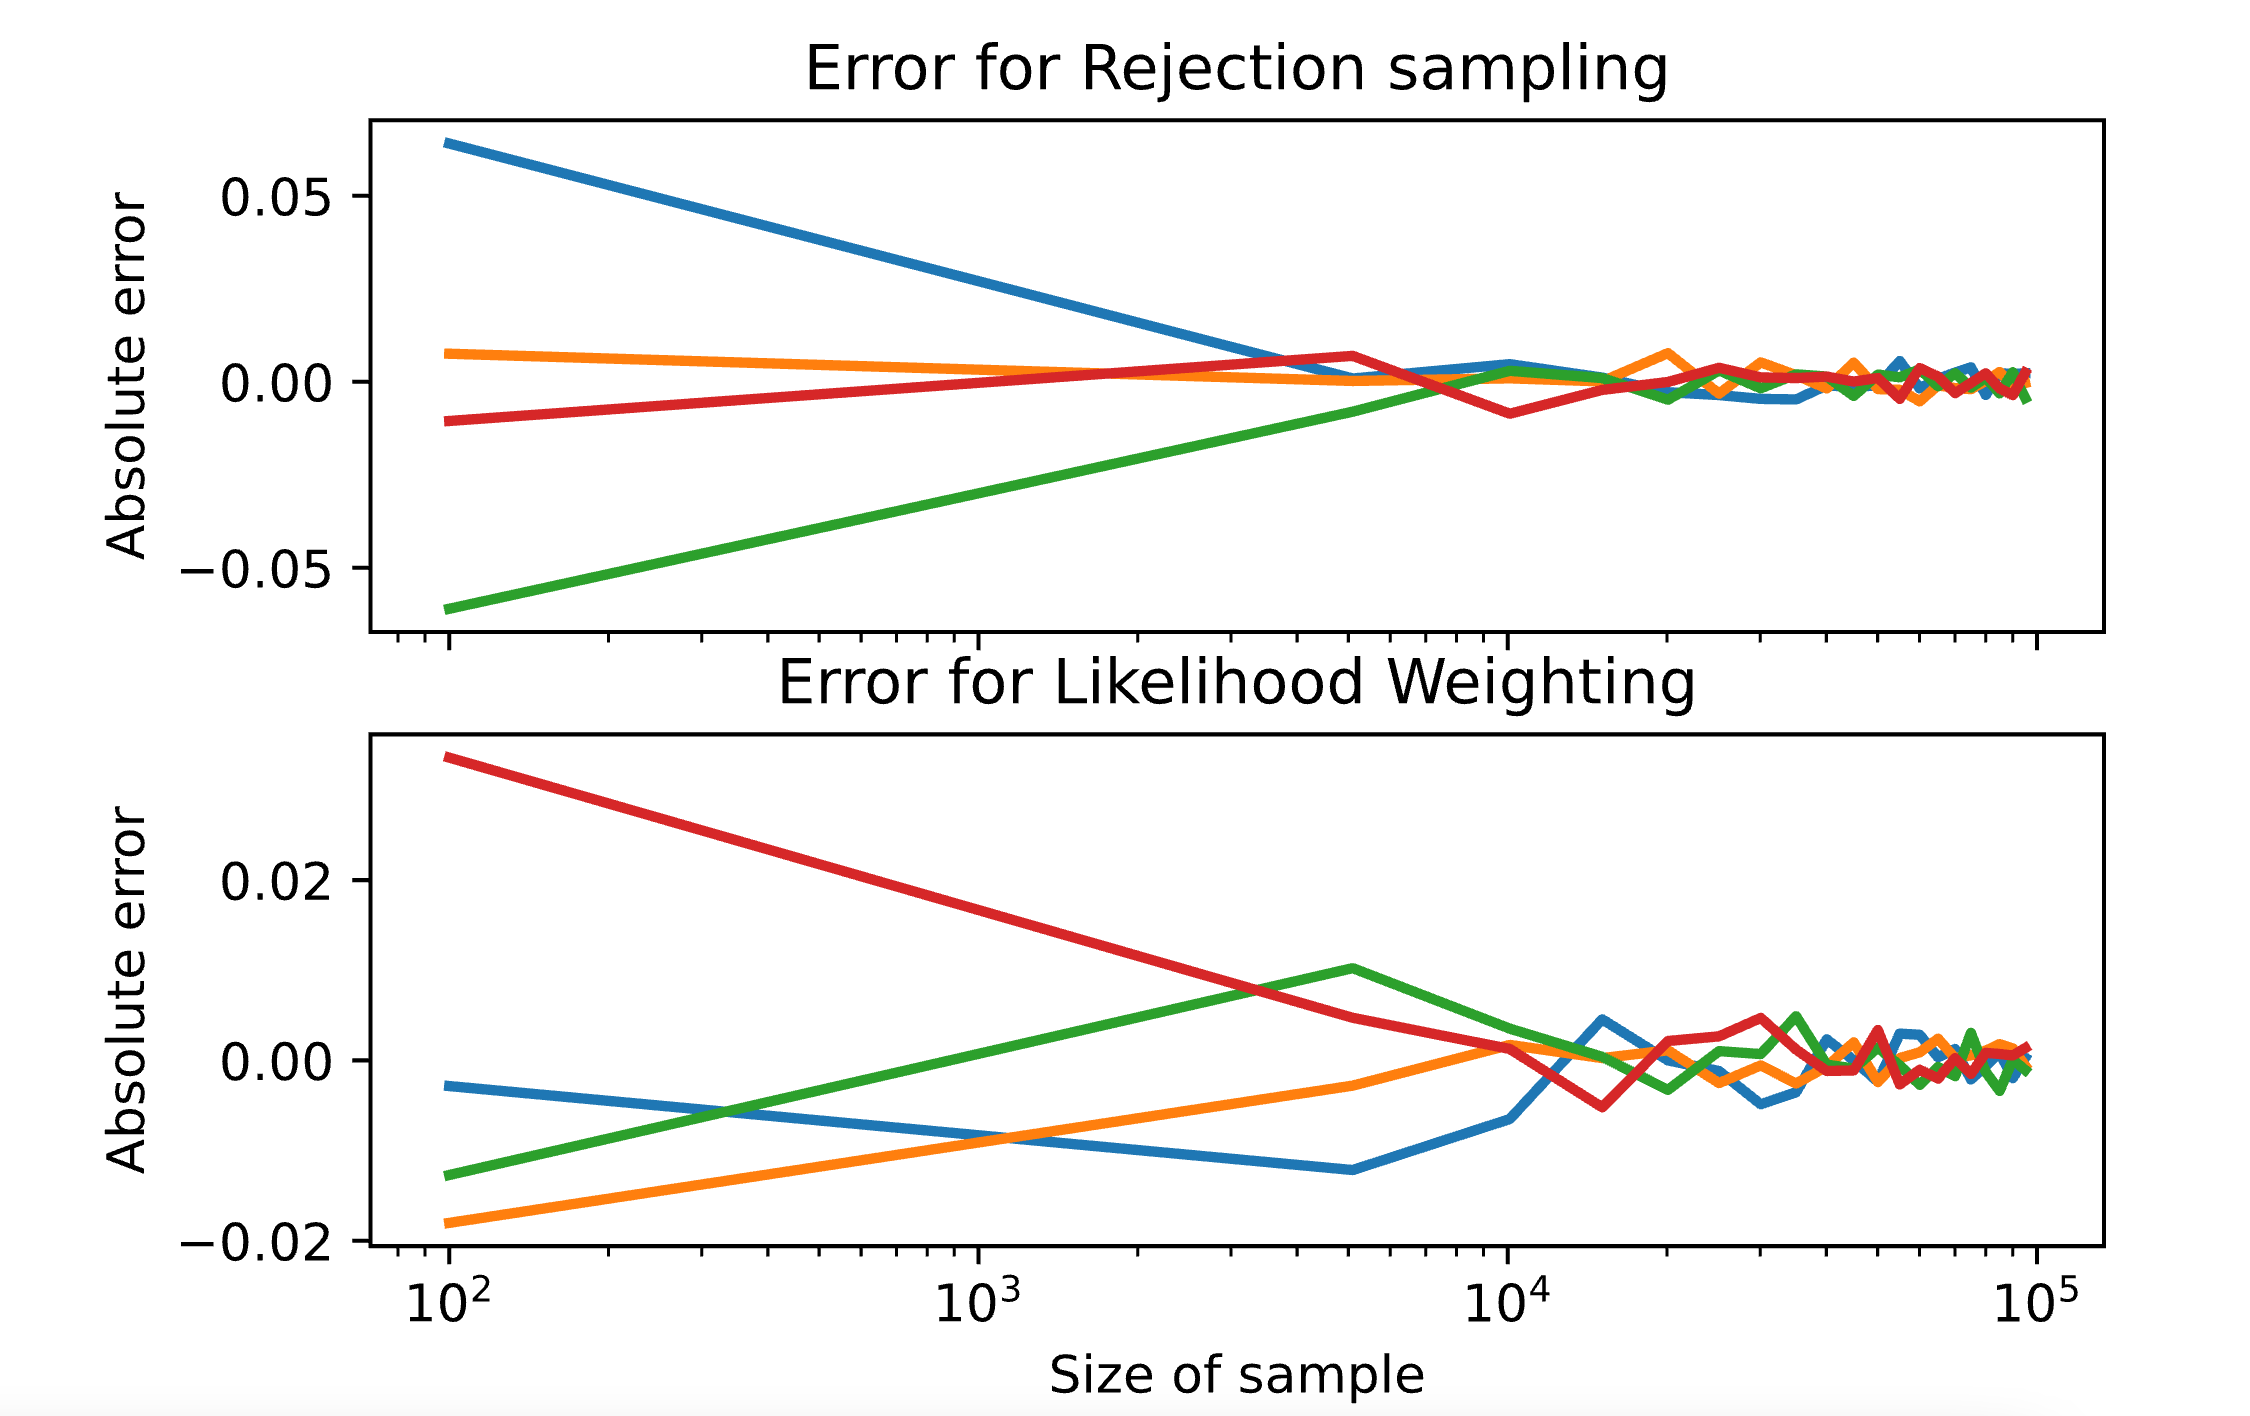
\includegraphics[width=0.8\linewidth]{figures/errors.png}
    \caption{Errors achieved on each acceptability class for the two algorithms.}
    \label{fig:errors}
\end{figure}
